\chapter{Apéndice A: Esquemáticos}
    El circuito Rev-Control Version 2.6 es un sistema de monitoreo y control de parámetros de un motor, diseñado para la medición y alerta de varias variables como RPM, presión de aceite, temperatura y concentración de oxígeno. Este sistema emplea un microcontrolador LPC845 para gestionar las entradas y salidas de los sensores y se conecta mediante un puerto micro-USB. Utiliza múltiples termocuplas, termistores y sensores específicos conectados a través de amplificadores para cada medición.\\

\begin{enumerate}
    \item \textbf{Microcontrolador LPC845}: Procesa las señales y controla el encendido de alertas. Cuenta con múltiples pines asignados a diferentes sensores y señales de salida.

    \item \textbf{Sensores de Temperatura - Termocuplas (MAX6675)}: Las termocuplas están distribuidas en varias posiciones del sistema para medir temperaturas en puntos específicos, con salidas gestionadas a través de los pines PIO0 del microcontrolador.

    \item \textbf{Sensores de Temperatura - Termistores (MAX31865)}: El MAX31865 convierte las señales de los termistores en datos procesables para el microcontrolador, permitiendo mediciones precisas en otras partes del sistema.

    \item \textbf{Sensor de Presión de Aceite}: Este sensor, conectado a los pines PIO0\_23 y PIO0\_01 del microcontrolador, mide la presión de aceite en el motor, operando en un rango de hasta 7 bar. Permite monitorear la lubricación adecuada del motor, activando alertas en caso de lecturas fuera del rango establecido.

    \item \textbf{Sonda Lambda (\%O2)}: Utiliza el amplificador operacional \textbf{LM358} para ajustar la señal de entrada de la sonda, que mide el nivel de oxígeno en los gases de escape. Indicadores visuales muestran el estado de la medición.

    \item \textbf{Regulador de Voltaje (LD1117D12)}: Proporciona una salida de 3.3V para alimentar componentes de bajo voltaje, asegurando una distribución estable de energía en el sistema.

    \item \textbf{Placa Step Down Regulada a 5V}: Regula la alimentación de 12V a 5V para los componentes que requieren esta tensión, proporcionando una fuente de energía estable y eficiente.

    \item \textbf{Potenciómetro y Resistencias}: Utilizados para calibrar y ajustar las señales de algunos sensores, como la señal de RPM.
\end{enumerate}


    \begin{landscape}
        \begin{sidewaysfigure}
            \centering
            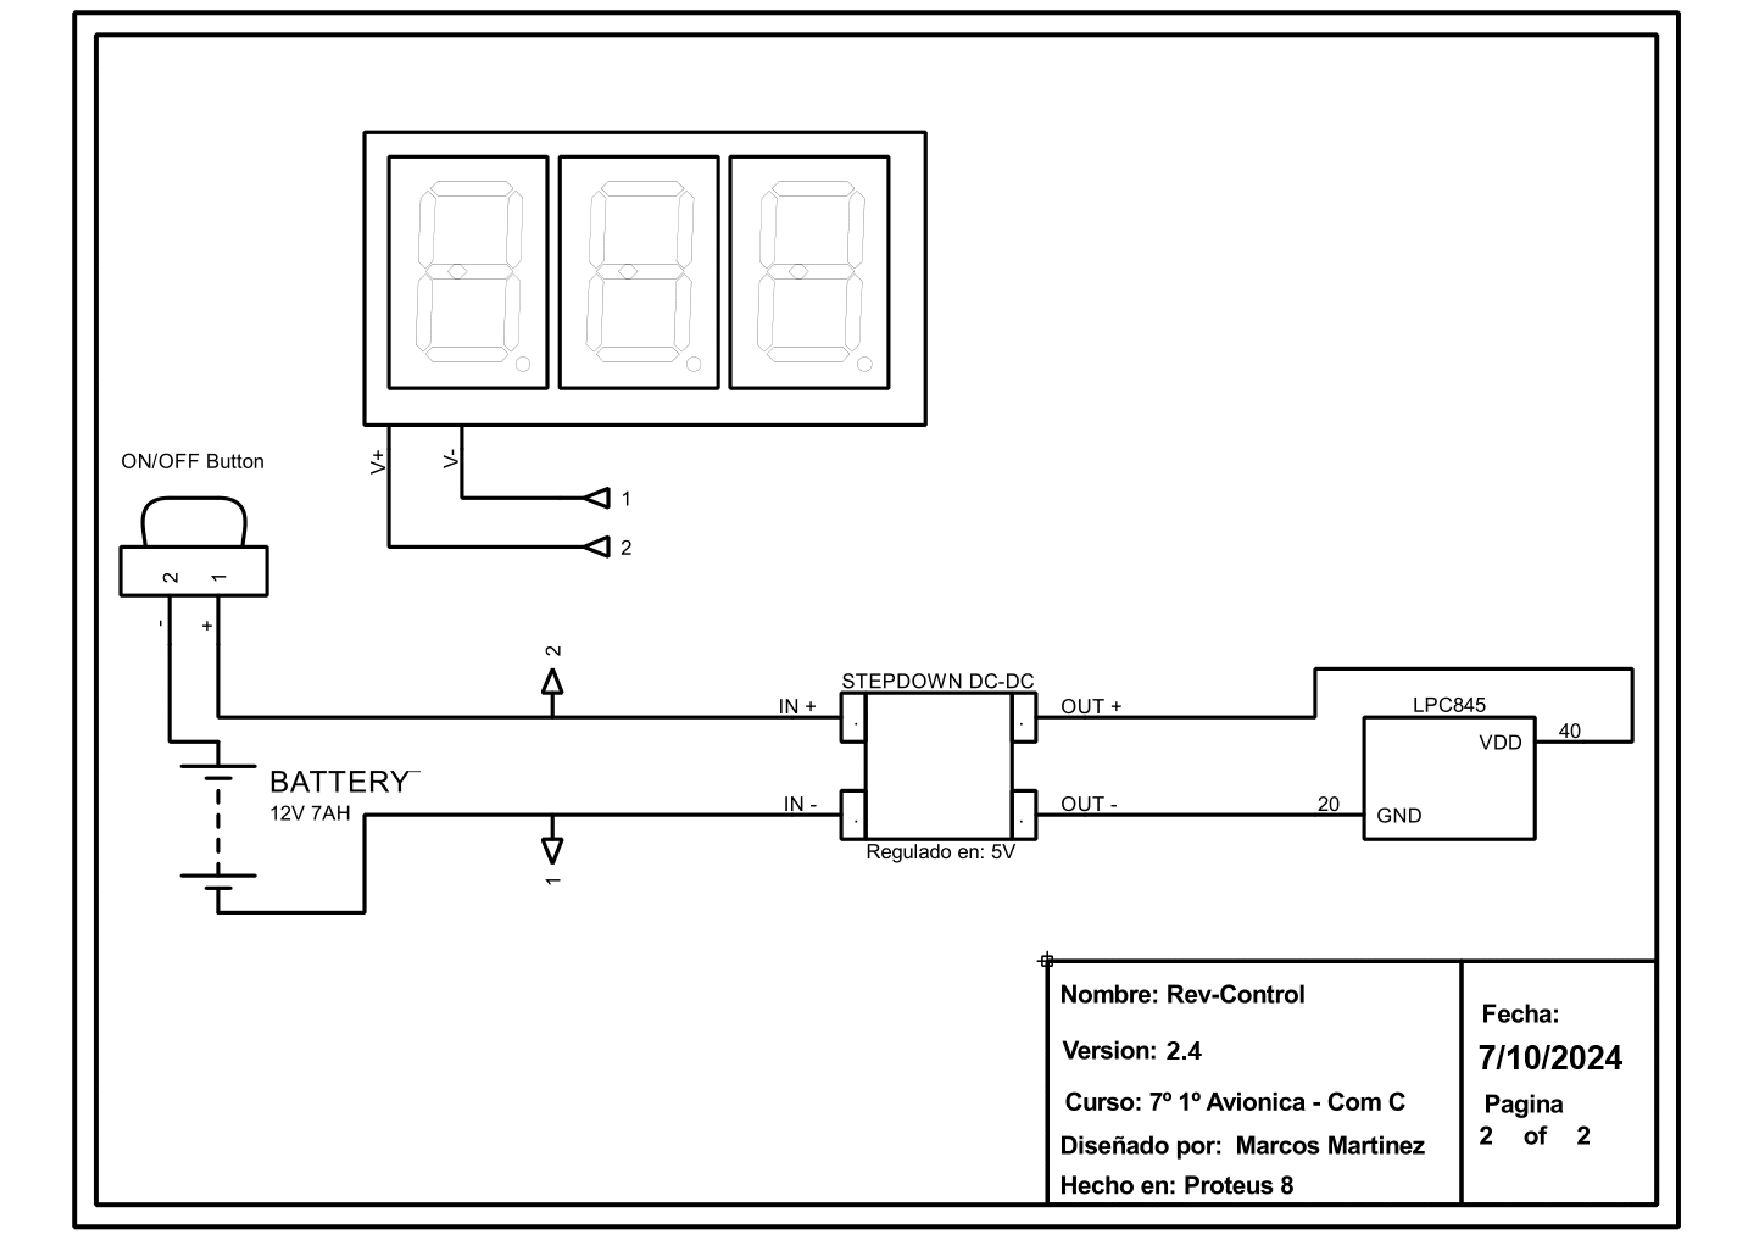
\includegraphics[angle=270, width=\textwidth, keepaspectratio]{Anexo-A Bloque/Rev- Control Version 2.4 Parte 2.pdf}
            \caption{Control Version 2.4 Parte 2}
            \label{fig:A_1}
        \end{sidewaysfigure}
        
        \newpage
        
        \begin{sidewaysfigure}
            \centering
            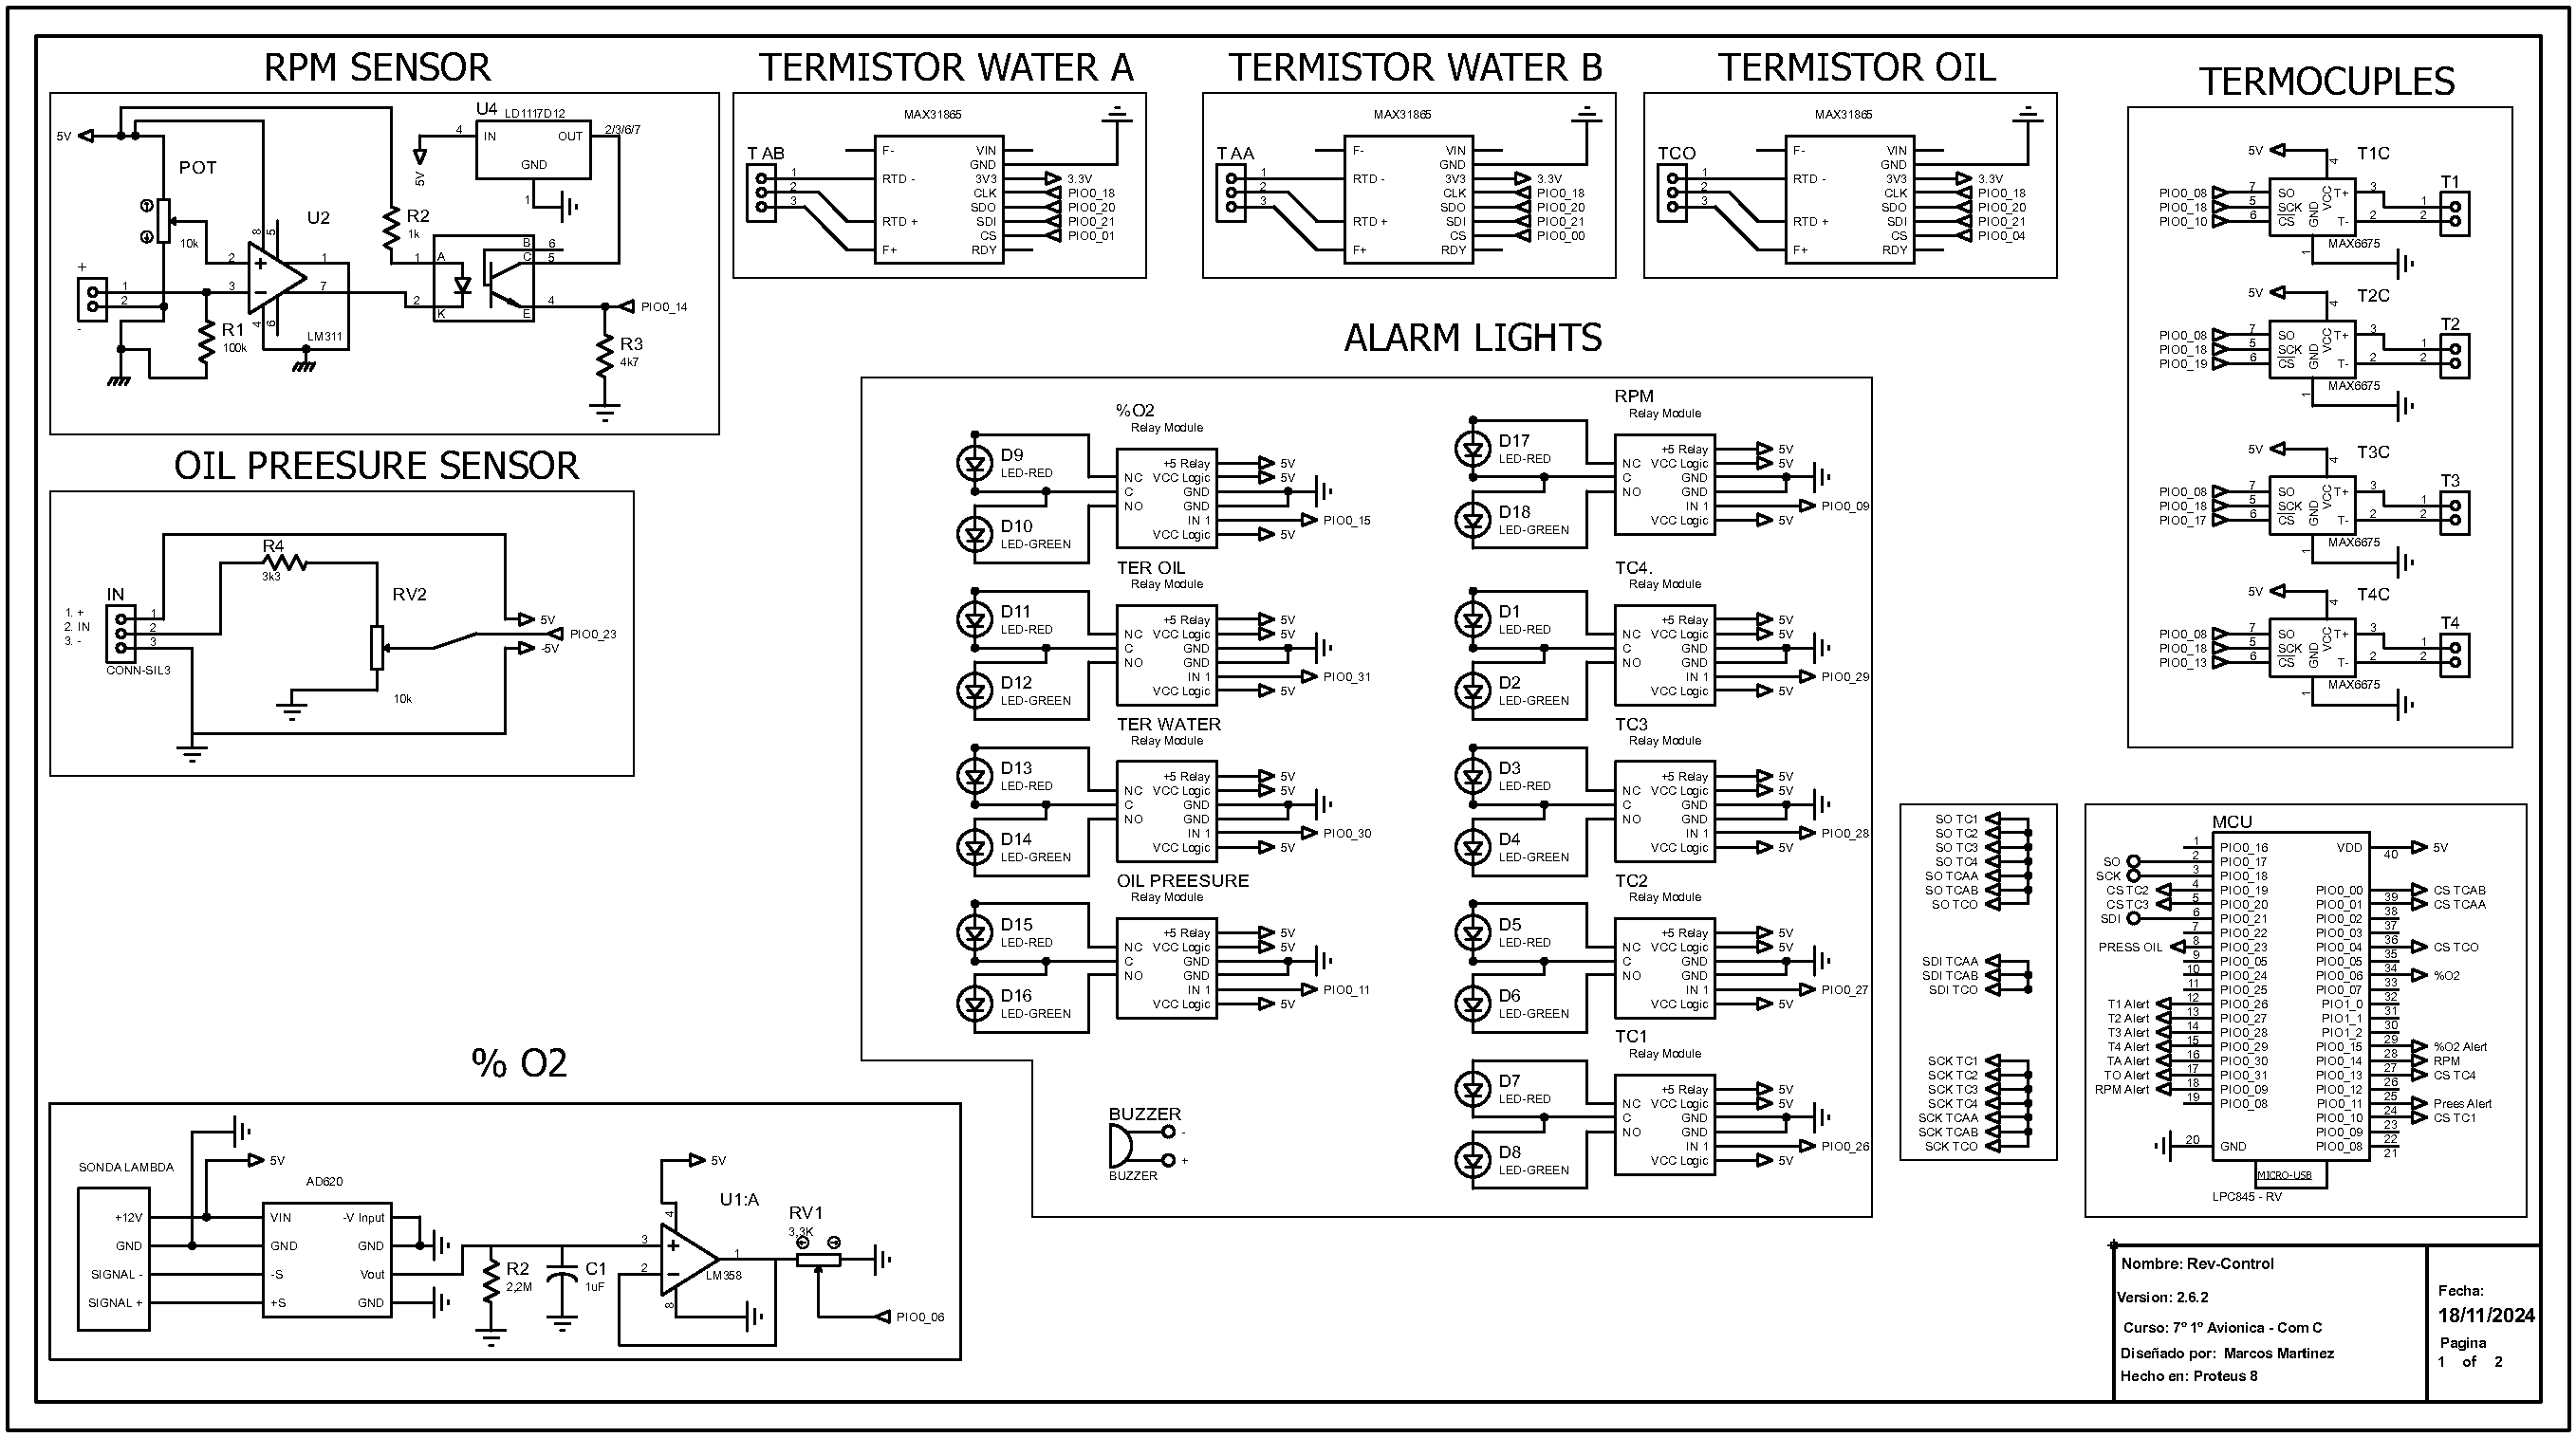
\includegraphics[angle=270, width=\textwidth, keepaspectratio]{Anexo-A Bloque/REV-CONTROL version2.6.2.PDF}
            \caption{Control Version 2.6}
            \label{fig:A_2}
        \end{sidewaysfigure}
        
    \end{landscape}